\documentclass[a2paper, 12pt]{article}
\usepackage[font={huge, bf}]{caption}
\usepackage{fontspec}
\setmainfont{Arial}
\usepackage{subcaption}
\usepackage{graphicx}
\usepackage{tikz}
\usepackage{tikzsymbols}
\usetikzlibrary{calc,patterns,shapes.geometric}
\usepackage{float}
\usepackage{pdflscape}
\usepackage{geometry}
\geometry{landscape, margin=2cm}
\captionsetup[subfigure]{justification=justified,singlelinecheck=false}
\pagestyle{empty}

\def\centerarc[#1](#2)(#3:#4:#5){\draw[#1] ($(#2)+({#5*cos(#3)},{#5*sin(#3)})$) arc (#3:#4:#5);}

\begin{document}
	\vspace*{\fill}
	\begin{figure}[!htbp]
		\centering
		\begin{subfigure}[b]{0.48\textwidth}
			\caption{Figure 1}
			\centering
			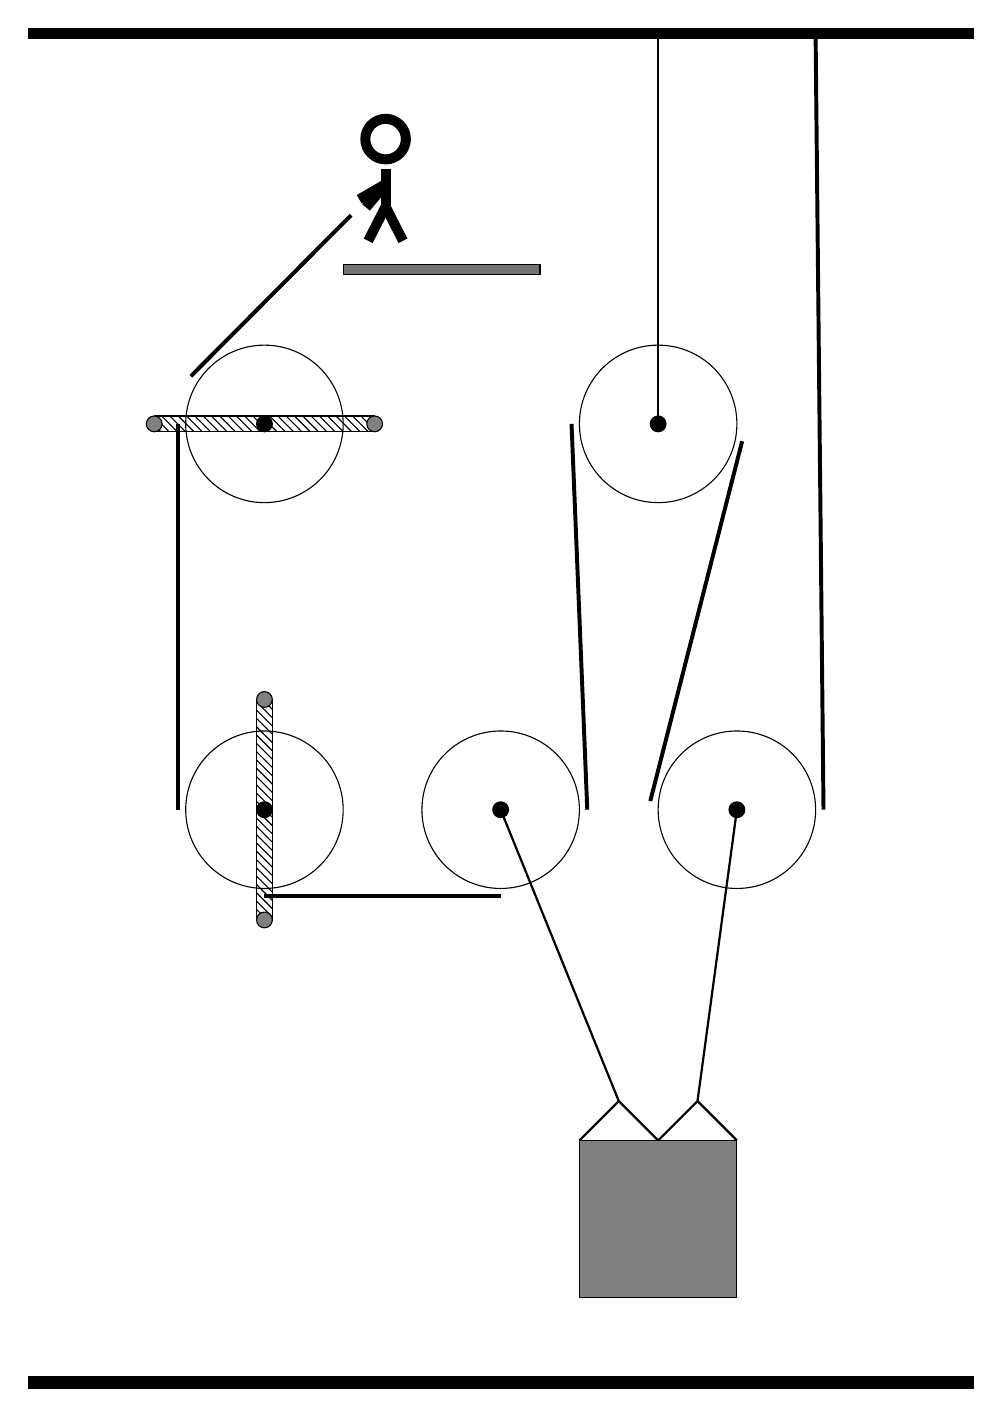
\begin{tikzpicture}
				\draw[fill=black] (-5, 14) rectangle (7, 14.125);
				
				\draw (1, 4.2) circle (1);
				\draw[fill=black] (1, 4.2) circle (0.1);
				
				\draw (3, 9.1) circle (1);
				\draw[fill=black] (3, 9.1) circle (0.1);
				\draw[thick] (3, 9.1) -- (3, 14);
				
				\draw (4, 4.2) circle (1);
				\draw[fill=black] (4, 4.2) circle (0.1);
				
				\draw[thick] (4, 4.2) -- (3.5, 0.5);
				\draw[thick] (1, 4.2) -- (2.5, 0.5);
				\draw[thick]  (2, 0) -- (2.5, 0.5) -- (3, 0);
				\draw[thick]  (3, 0) -- (3.5, 0.5) -- (4, 0);
				\draw[fill=black!50] (2, 0) rectangle (4, -2);
				
				\draw (-2, 4.2) circle (1);
				\draw[fill=black] (-2, 4.2) circle (0.1);
				\draw[pattern=north west lines, pattern color=black] (-2.1, 5.6) rectangle (-1.9, 2.8);
				\draw[fill=black!50] (-2, 5.6) circle (0.1);
				\draw[fill=black!50] (-2, 2.8) circle (0.1);
				
				\draw (-2, 9.1) circle (1);
				\draw[fill=black] (-2, 9.1) circle (0.1);
				\draw[pattern=north west lines, pattern color=black] (-3.4, 9.2) rectangle (-0.6, 9.0);
				\draw[fill=black!50] (-3.4, 9.1) circle (0.1);
				\draw[fill=black!50] (-0.6, 9.1) circle (0.1);
				
				\draw[line width=0.5mm] (-0.9, 11.75) -- (-2.935, 9.705);
				\centerarc[line width=0.5mm](-2, 9.1)(135:180:1.1);
				\draw[line width=0.5mm] (-3.1, 9.1) -- (-3.1, 4.2);
				\centerarc[line width=0.5mm](-2, 4.2)(180:270:1.1);
				\draw[line width=0.5mm](-2, 3.1) -- (1, 3.1);
				\centerarc[line width=0.5mm](1, 4.2)(270:360:1.1);
				\draw[line width=0.5mm] (2.1, 4.2) -- (1.9, 9.1);
				\centerarc[line width=0.5mm](3, 9.1)(-20:180:1.1);
				\draw[line width=0.5mm](4.067, 8.88) -- (2.9, 4.31);
				\centerarc[line width=0.5mm](4, 4.2)(160:360:1.1);
				\draw[line width=0.5mm](5.1, 4.2) -- (5.0, 14);
				
				\node at (-0.5, 12.2) {\scriptsize \Strichmaxerl[10][30][-130]};
				\draw[fill=black!55] (-1.0, 11) rectangle (1.5, 11.125);
				
				\draw[fill=black] (-5, -3) rectangle (7, -3.15);
			\end{tikzpicture}
		\end{subfigure}
		\hfill
		\begin{subfigure}[b]{0.48\textwidth}
			\caption{Figure 2}
			\centering
			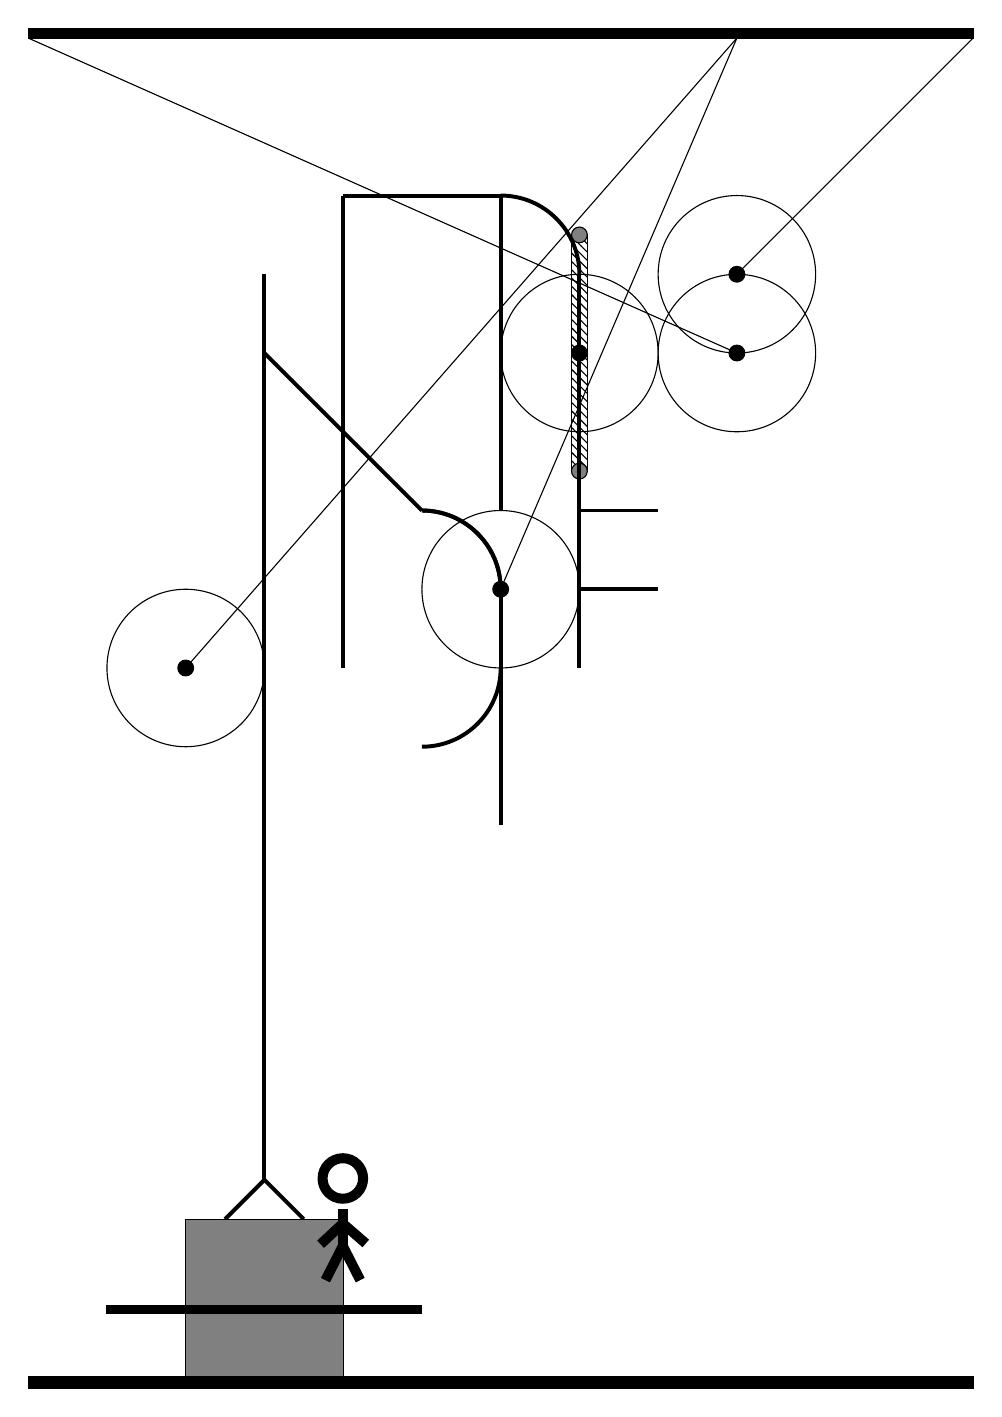
\begin{tikzpicture}
				\draw[fill=black] (-5, 14) rectangle (7, 14.125);
				
				\draw (1,7) circle (1);
				\draw[fill=black] (1,7) circle (0.1);
				\draw (4,14.0) -- (1,7);
				
				\draw (-3,6) circle (1);
				\draw[fill=black] (-3,6) circle (0.1);
				\draw (4,14.0) -- (-3,6);
				
				\draw (2,10) circle (1);
				\draw[fill=black] (2,10) circle (0.1);
				\draw[pattern=north west lines, pattern color=black] (1.9,11.5) rectangle (2.1,8.5);
				\draw[fill=black!50] (2,11.5) circle (0.1);
				\draw[fill=black!50] (2,8.5) circle (0.1);
				
				\draw (4,10) circle (1);
				\draw[fill=black] (4,10) circle (0.1);
				\draw (-5,14.0) -- (4,10);
				
				\draw (4,11) circle (1);
				\draw[fill=black] (4,11) circle (0.1);
				\draw (7,14.0) -- (4,11);
				
				\draw[line width=0.5mm](-2,-0.5) -- (-2,11.0);
				\draw[line width=0.5mm](-2.5,-1) --  (-2,-0.5) -- (-1.5,-1);
				\draw[fill=black!50] (-3, -1) rectangle (-1, -3);
				
				\draw[line width = 0.5mm] (1,4) -- (1,7);
				\draw[line width = 0.5mm] (0,8) arc (90:0:1);
				\draw[line width = 0.5mm] (0,8) -- (-2,10);
				\draw[line width = 0.5mm] (-1,6) -- (-1,11);
				\centerarc[line width = 0.5mm](0,11)(0:180:1);
				\draw[line width = 0.5mm] (1,11) -- (1,8);
				\centerarc[line width = 0.5mm](2,8)(270:180:1);
				\draw[line width = 0.5mm] (2,7) -- (3,7);
				\draw[line width = 0.5mm] (0,5) arc (270:360:1);
				\draw[line width = 0.5mm] (1,6) -- (1,7);
				\draw[line width = 0.5mm] (1,7) arc (0:90:1);
				\draw[line width = 0.5mm] (2,6) -- (2,11);
				\draw[line width = 0.5mm] (1,12) arc (90:0:1);
				\draw[line width = 0.5mm] (1,12) -- (-1,12);
				\draw[line width = 0.5mm] (-1,7) -- (-1,12);
				\centerarc[line width = 0.5mm](0,12)(0:180:1);
				\draw[line width = 0.5mm] (1,12) -- (1,9);
				\centerarc[line width = 0.5mm](2,9)(270:180:1);
				\draw[line width = 0.5mm] (2,8) -- (3,8);
				
				\node at (-1, -1) {\scriptsize \Strichmaxerl[10][43][-41]};
				\draw[fill=black] (-4, -2.1) rectangle (0, -2.2);
				
				\draw[fill=black] (-5, -3) rectangle (7, -3.15);
			\end{tikzpicture}
		\end{subfigure}
	\end{figure}
		\vspace*{\fill}
\end{document}